\chapter{Обзор существующих технологий бинарной трансляции}\label{ch:ch1}
Первая глава содержит обзор существующих технологий бинарных трансляторов, используемых для генерации оптимизированных исполняемых файлов приложений.

В разделе 1.1 приводится описание методов оптимизаций приложений.

В разделе 1.2 рассматриваются общие принципы работы существующих технологий бинарных оптимизаторов и приводится обзор на существующие решения.

В разделе 1.3 подробно рассматривается устройство бинарного оптимизатора BOLT (Binary Optimization and Layout Tool), вопросы получения профильной информации для его работы на x86 архитектуре с использованием аппаратной поддержки профилирования -- LBR (Last Branch Record).

Разбираются вопросы формата профилей с информацией о взятых переходах и без неё и пример оптимизации простого приложения с условным переходом в цикле.

В конце первой главы обсуждается вопрос поддержки архитектуры ARM в бинарном оптимизаторе BOLT, варианты получения профильной информации на ней и возможности оптимизаций. Приведены примеры профилей в формате BOLT.

\section{Процесс оптимизации приложений}\label{sec:ch1/sec1}
На данный момент большинство программ пишутся на языке программирования высокого уровня, после чего применяются трансляторы, переводящие их в бинарный формат (рисунок \cref{fig:TransVar}). Так называемые программирующие программы (компиляторы) появились ещё в 50-х годах двадцатого века.

\begin{figure}[!h]
    \centerfloat{
        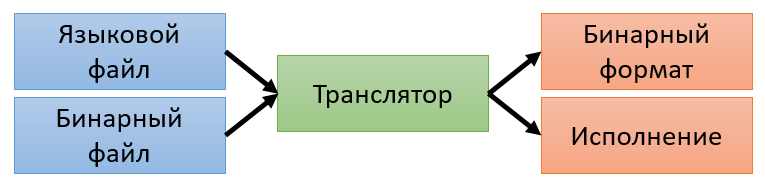
\includegraphics[width=0.8\linewidth]{translate1}
    }
    \caption{Варианты работы транслятора}\label{fig:TransVar}
\end{figure}

Практически всегда приложение проходит процесс оптимизации во время компиляции, так как данные проходы включают в системах сборки по умолчанию. Во время трансляции программы с языка высокого уровня в бинарный код реальной или виртуальной машины получаемое промежуточное представление подвергается упорядоченному набору оптимизаций. Для компилируемых языков применяются дополнительные оптимизации времени компоновки кода (LTO – Link Time Optimizations), поскольку на этом этапе становится доступно больше информации о всех полученных объектных файлах. После компоновки кода приложение готово к использованию \cite{Wu1994}. Для данных оптимизаций использовалась информация о приложении, полученная из исходного кода.

Для повышения производительности можно собрать профиль исполнения приложения, что позволит лучше подобрать эвристики для используемых оптимизационных проходов, а также применить дополнительные проходы в компиляторе и линкере \cite{Licker2020}.

\section{Бинарная оптимизация}\label{sec:ch1/sec2}
В случае, когда доступа к исходному коду нет, но есть бинарный файл приложения и его профиль исполнения, появляется возможность провести бинарную оптимизацию\cite{Li2019}. Тогда на вход транслятору будет подаваться не языковой, а бинарный файл (рисунок \cref{fig:TransVar}), который будет переведён в другой бинарный формат.

Целевая архитектура для входного и выходного формата могут не совпадать. В случае их совпадения целесообразно использовать данный транслятор с оптимизациями под конкретную модель процессора. Добавив информацию о его спецификации, на котором будет исполнятся приложение, можно провести ряд микроархитектурных оптимизаций. Также можно использовать профильную информацию исполнения для проведения дополнительных оптимизирующих проходов.

За последние несколько лет наблюдается резкий рост популярности бинарных оптимизаторов: BOLT \cite{Panchenko2019}, Propeller \cite{Moreira2021}, Janus \cite{Zhou2019}, HALO \cite{Savage2020}, Ispike \cite{Luk2004}. Эти инструменты используют профильную информацию исполнения для принятия решений по оптимизации.

Оптимизация, основанная на обратной связи (FDO, Feedback Directed Optimization), является эффективным методом повышения производительности программ сверх того, что обычно могут достичь статические компиляторы \cite{Chen2016}. В данном сценарии компилятор использует информацию, полученную в результате предыдущих исполнений целевой программы, для выполнения более агрессивных преобразований кода. FDO является ключевым компонентом инструментов бинарной оптимизации, которые полагаются на информацию профилирования для выполнения преобразований, таких как изменение порядка базовых блоков и функций.
Эти инструменты достигают прироста производительности благодаря оптимизации с профилем исполнения: BOLT (Binary Optimization and Layout Tool) \cite{Panchenko2019} дает ускорение приложений до 30\% (при отсутствии предварительных профильных оптимизаций).

Несмотря на эффективность, сбор данных во время выполнения создает разработчикам неудобства: подбор входных данных, необходимость внесения изменений в программное обеспечение и увеличение времени сборки.

Помимо генерации бинарного файла, транслятор может произвести исполнение считанного им кода на высокоуровневом языке программирования либо бинарном формате. В первом случае это будет интерпретацией, во втором - моделированием/бинарной интерпретацией, что позволяет проводить тестовые запуски без наличия реального устройства.

\section{Обзор бинарного оптимизатора BOLT}\label{sec:ch1/sec3}
Основными целевыми приложениями для оптимизатора BOLT являются современные программы для центров обработки данных. Из-за размера кода программ повышение его локализации стало важным инструментом повышения производительности \cite{Ottoni2017}. Основной оптимизацией BOLT является перекомпоновка кода на основе полученного профиля, использование которого на бинарном уровне точнее, чем на этапе компиляции (рисунок \cref{fig:BOLT}) \cite{Newell2020}. Создатели данного бинарного оптимизатора достигли прироста производительности в 10\% на x86 приложениях, скомпилированные с оптимизациями времени связывания и с использованием профиля \cite{Panchenko2019}\cite{Panchenko2021}.

\begin{figure}[!h]
    \centerfloat{
        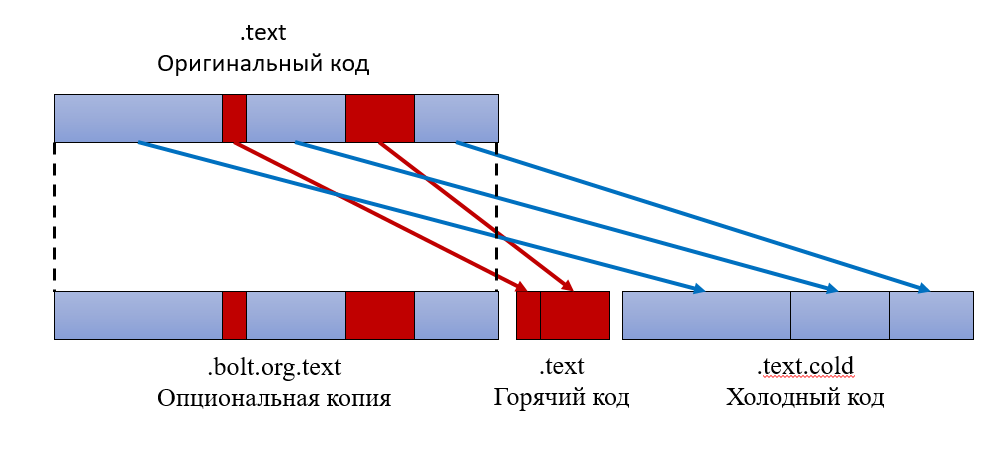
\includegraphics[width=1.0\linewidth]{1}
    }
    \caption{Алгоритм работы бинарного оптимизатора BOLT}\label{fig:BOLT}
\end{figure}

Данный бинарный оптимизатор написан с использованием фреймворка генерации компиляторов – LLVM \cite{Lattner2004}, что делает BOLT потенциально портируемым на множество других архитектур. Базовая поддержка ARM архитектуры (Aarch64) на данный момент уже добавлена.

BOLT применим к приложениям, размер которых значительно больше размера L1I (инструкционного кэша 1 уровня) и размера отображаемого кода iTLB (буфер ассоциативной трансляции инструкций) - десятки мегабайт и более. За счет новой компоновки кода, основанной на профиле, часто исполняемый код локализуется в новой секции. Частоту исполнения кода называют его <<температурой>>, и в данном примере созданная секция является <<горячей>>. Остальной же код с меньшей частотой исполнения будет называться <<холодным>>. Теперь при обращении в горячий участок кода в кэш-линию, помимо исполняемого в данный момент кода, будут попадать более горячие соседние участки из новой секции, и температура кода инструкционного кэша будет выше \cite{Lavaee2019}. Это приводит к меньшим промахам при обращении в L1I и iTLB, а значит к повышению производительности.

Для оптимизации с помощью BOLT необходима релокационная информация, так как его алгоритм производит перекомпоновку всей секции .text, в которой может содержаться как код, так и данные. Это одна из особенностей фон-Неймановских архитектур: код и данные располагаются в одном адресном пространстве.

На рисунке \cref{fig:4byte} представлен пример, когда одни и те же 4-байтовые данные могут обозначать либо ARM инструкцию условного перехода, либо 4 символа. При перекомпоновке необходимо изменить значение смещения инструкции b.ls, во втором случае 4-байтовые данные должны остаться неизменными, поэтому без дополнительной информации о расположении данных оптимизатор не сможет решить, как обработать секцию корректно. 

\begin{figure}[!h]
    \centerfloat{
        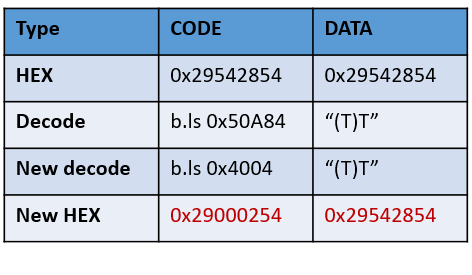
\includegraphics[width=0.7\linewidth]{12}
    }
    \caption{Пример модификации 4-байтовых данных при перемещении кода}\label{fig:4byte}
\end{figure}

Помимо релокационной информации BOLT требует наличие символов в бинарном файле, так как он оперирует с бинарными функциями. Также формат профиля в BOLT использует имена символов для обозначения местоположения инструкций переходов.

\subsection{Получение профильной информации для оптимизатора BOLT}\label{subsec:ch1/sec3/sub1}
Один из способов собрать профиль – провести инструментацию бинарного файла \cite{Ottoni2018}. Во время запуска будет произведена запись по счетчикам, расставленным во время компиляции, но для данного подхода необходим исходный код. Основная проблема заключается в необходимости адаптации инфраструктуры сборки проекта для профилирования. Кроме того, используемые сторонние библиотеки не предоставляются в инструментированном виде, что осложняет получения полной картины исполнения \cite{Nethercote2007}.

Вместо инструментации кода во время компиляции разработаны среды, позволяющие произвести инструментацию во время исполнения приложения. Таким образом, может быть получена вся необходимая информация об исполнении при разрешении сложностей извлечения собранных данных. Однако, стоимость разработки динамической инструментации выше разработки аналогичного процесса в момент компиляции. Также появляются затраты вычислительных ресурсов во время записи трасс исполнения.\cite{Li2007}

При наличии архитектурной поддержки есть возможность собрать информацию исполнения с меньшими расходами. В x86 архитектуре такая поддержка есть, что позволило сотрудникам Facebook использовать такой подход в своём бинарном оптимизаторе BOLT (рисунок \cref{fig:OptX86})\cite{Panchenko2019}.

\begin{figure}[!h]
    \centerfloat{
        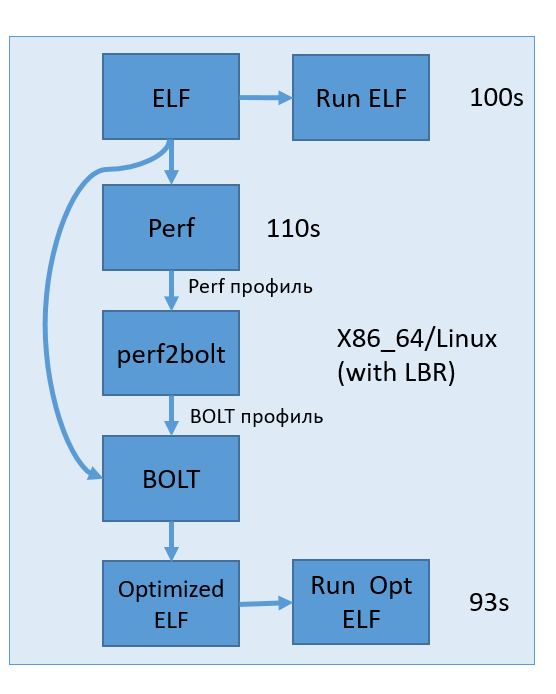
\includegraphics[width=0.6\linewidth]{2}
    }
    \caption{Схема оптимизации бинарного файла на x86 архитектуре}\label{fig:OptX86}
\end{figure}

Для нахождения горячих и холодных участков кода используется профиль (рисунок \cref{fig:ProfileFormat}), собранный на основе выборок. BOLT использует данные, полученные с помощью приложения perf, собирающее статистические данные исполнения, такие как значения счетчика команд и последние взятые переходы с информацией от предсказателя переходов. Последний параметр предоставляется perf благодаря аппаратной поддержке в архитектуре x86. Поддержка осуществляется с помощью LBR (Last Branch Record), записывающей информацию о последних 8-32 (в зависимости от модели процессора) переходах.

\begin{figure}[!h]
    \centerfloat{
        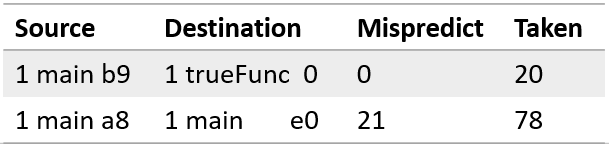
\includegraphics[width=0.8\linewidth]{profile}
    }
    \caption{Формат профильной информации бинарного оптимизатора BOLT}\label{fig:ProfileFormat}
\end{figure}

Сначала идет информация о местонахождении инструкции перехода (Source). Это поле задается тремя значениями: является ли дальнейшее поле символом (0 или 1), имя символа в исполняемом файле, смещение от символа  до инструкции перехода. Далее в такой же последовательности следует информация о месте назначения прыжка (Destination). Последние два числа – количество не предсказанных и количество взятых переходов.
	На рисунке \cref{fig:ProfileFormat} продемонстрирована информация о двух переходах:
	
\begin{enumerate}[beginpenalty=10000]
  \item Вызов trueFunc из main, являющийся прямым прыжком (поэтому mispredict = 0), взятый 20 раз.
  \item Переход внутри функции main, который является условным прыжком, не предсказанный 21 раз и взятый 78 раз.
\end{enumerate}

Затем происходит конвертация профиля из формата perf в формат BOLT при помощи приложения perf2bolt. В итоге будет сгенерирован список записей, состоящих из адресов начала и конца перехода, количества не предсказанных и количества взятых переходов.

На основании полученного профиля начинается работа бинарного оптимизатора. На рисунке \cref{fig:BinOptSteps} представлена схема работы BOLT.

\begin{figure}[!h]
    \centerfloat{
        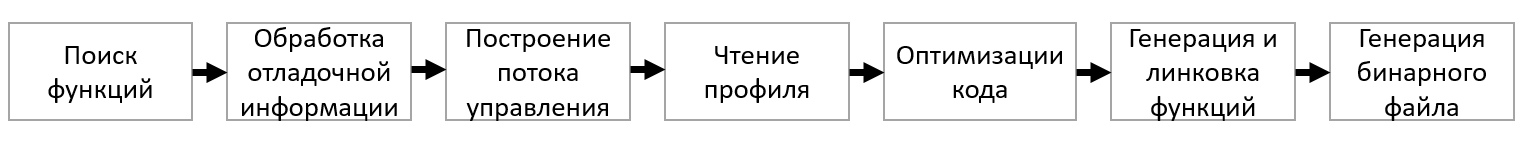
\includegraphics[width=1.0\linewidth]{3}
    }
    \caption{Последовательность работы бинарного оптимизатора BOLT}\label{fig:BinOptSteps}
\end{figure}

Уровни абстракций, на которых работает BOLT, выстраиваются в последовательности, показанной на рисунке \cref{fig:BOLTAbst}.

\begin{figure}[!h]
    \centerfloat{
        
\includegraphics[width=1.0\linewidth]{4}
    }
    \caption{Уровни абстракции бинарного оптимизатора BOLT}\label{fig:BOLTAbst}
\end{figure}

Для первых 4 абстракций создатели BOLT написали в программном коде свои собственные классы. Машинные инструкции были использованы из стандартных классов LLVM (MCInst). Под бинарным базовым блоком понимается линейный участок кода, исполнение которого всегда идёт с его первой инструкции и заканчивается последней.

После работы бинарного оптимизатора получается новый бинарный файл, в котором вместо одной секции .text с исходным кодом появляется две секции .text (с горячим кодом) и .text.cold (с холодным кодом).
	
BOLT поддерживает возможность сохранения оригинальной секции. В таком случае он переименует её в .bolt.org.text. Это необходимо для тех случаев, когда перенос некоторых бинарных функций невозможен и необходимо переиспользовать оригинальный код.


\subsection{Пример оптимизации}\label{subsec:ch1/sec3/sub2}

Рассмотрим пример оптимизации следующей функции main (рисунок \cref{fig:TestCode}).

\begin{figure}[!h]
    \centerfloat{
        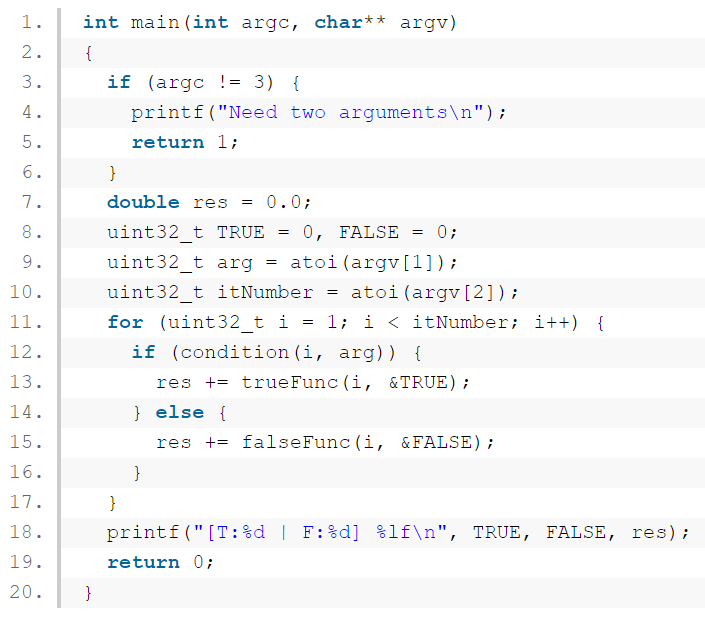
\includegraphics[width=0.8\linewidth]{5}
    }
    \caption{Пример оптимизируемого демонстрационного приложения}\label{fig:TestCode}
\end{figure}

BOLT найдёт символ main в таблице символов, перейдёт по указанному адресу в бинарном файле, дизассемблирует тело функции и выстроит поток управления данной функции (рисунок \cref{fig:CFG}).

\begin{figure}[!h]
    \centerfloat{
        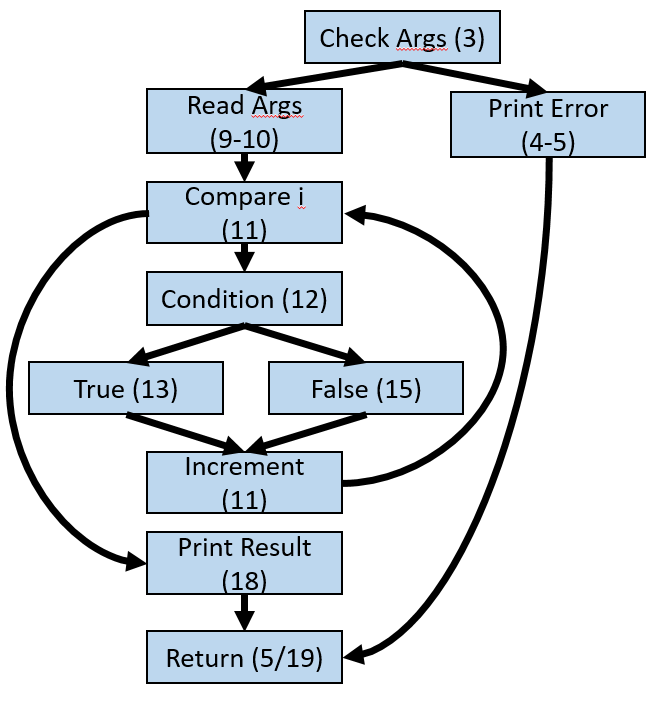
\includegraphics[width=0.6\linewidth]{6}
    }
    \caption{Граф потока управления (в скобках соответствующие строки кода)}\label{fig:CFG}
\end{figure}

Каждому узлу в графе потока управления соответствует один бинарный базовый блок, которым будет оперировать BOLT. При компиляции без профильной информации компилятор размещает код последовательно в одной .text секции, как указано на рисунке \cref{fig:BBOpt} слева. После запуска программы с профилировщиком на конкретных аргументах получим следующий профиль (рисунок \cref{fig:CFGProfile}).

\begin{figure}[!h]
    \centerfloat{
        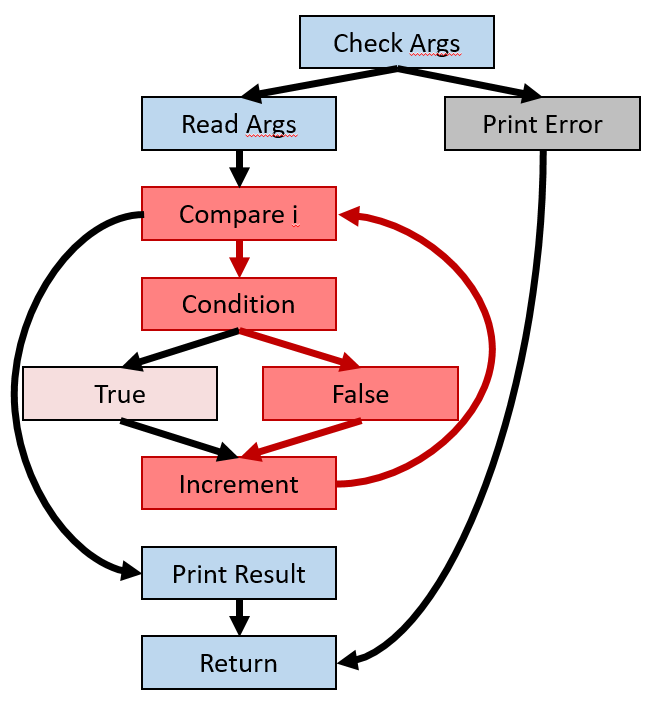
\includegraphics[width=0.6\linewidth]{7}
    }
    \caption{Граф потока управления с профильной информацией}\label{fig:CFGProfile}
\end{figure}

С учетом полученной информации от профилировщика известна частота исполнения базовых блоков, размещенных в бинарном файле (рисунок \cref{fig:BBOpt}, в центре). Получается, что самый часто исполняемый (горячий код) разбит холодным бинарным базовым блоком True, который будет попадать в кэш-линию при копировании кода в L1I и понижать его среднюю температуру.

\begin{figure}[!h]
    \centerfloat{
        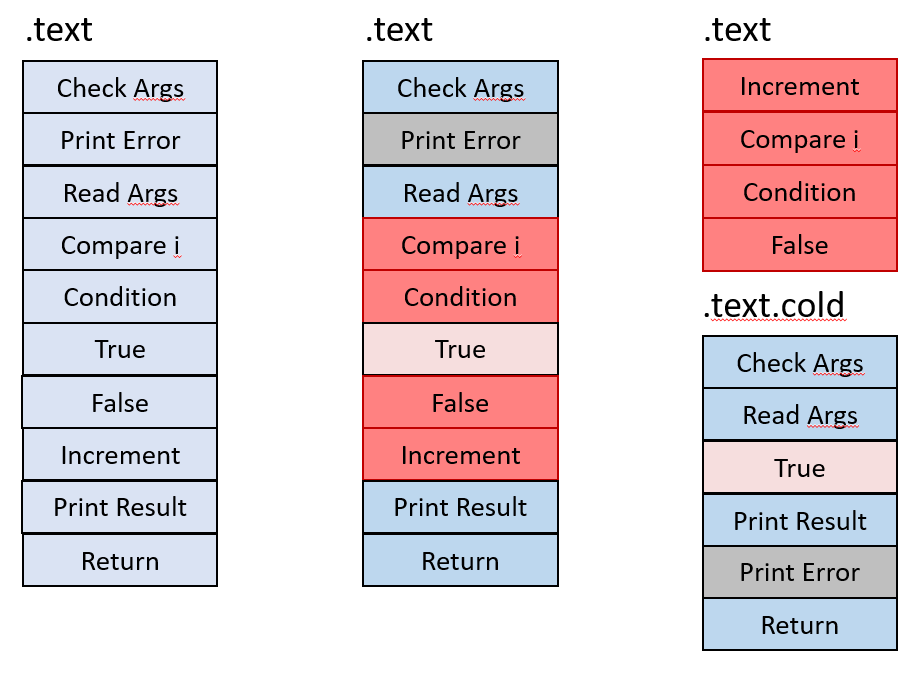
\includegraphics[width=0.8\linewidth]{8}
    }
    \caption{Расположение базовых блоков в секции (без профильной информации – с профильной информацией – после перекомпоновки кода)}\label{fig:BBOpt}
\end{figure}

Оптимизация BOLT переставляет бинарные базовые блоки (рисунок \cref{fig:BBOpt}, справа). Самые горячие блоки попадут в горячую секцию .text, остальные будут скопированы в секцию .text.cold. В итоге за счёт повышения средней температуры L1I  и iTLB полученный бинарный файл будет работать быстрее.

Как было сказано раньше, основной архитектурой для оптимизации была заявлена x86. Также заявлена поддержка 64-битной ARM архитектуры (Aarch64), но на деле возникает множество проблем при попытке использования оптимизатора на ней. Они будут рассмотрены в следующих разделах.


\subsection{Результаты тестирования BOLT на архитектуре x86}\label{subsec:ch1/sec3/sub3}
Для приведенного кода (рисунок \cref{fig:TestCode}) был получен профиль на x86 архитектуре с (таблица \cref{tab:X86LBR}) и без (таблица \cref{tab:X86noLBR}) информацией о взятых переходах из LBR.

no\_LBR\_mode – режим сбора статистики без LBR, в котором профильная информация включает в себя только количество исполнений конкретных инструкций.
\begin{table} [!h]% Пример записи таблицы с номером, но без отображаемого наименования
    \centering
    \begin{threeparttable}% выравнивание подписи по границам таблицы
        \caption{Профиль демонстрационного примера на x86 архитектуре, собранного с учетом информации из LBR}%
        \label{tab:X86LBR}%
        \begin{SingleSpace}
            \begin{tabular}{| c | c | c | c | c | c | c | c |}
                \hline
                	1 & main &      75 & 1 & main &      7b & 0 &   452 \\ \hline
				1 & main &      9e & 1 & main &      a4 & 0 &   421 \\ \hline
				1 & main &      ec & 1 & main &      f1 & 0 &   331 \\ \hline
				1 & main &      e2 & 1 & falseFunc & 0 &  0 &   665 \\ \hline
				1 & main &      c8 & 1 & main &      f1 & 0 &   98 \\ \hline
				1 & main &      9e & 1 & main &      cd & 317 &  730 \\ \hline
				1 & main &      b9 & 1 & trueFunc &  0 &  0 &   159 \\ \hline
				1 & main &      f1 & 1 & main &      f6 & 0 &   494 \\ \hline
				1 & main &      96 & 1 & condition & 0 &  0 &   4535 \\ \hline
				1 & main &      ff & 1 & main &      6e & 0 &   490 \\ \hline
				1 & main &      8c & 1 & atoi@PLT &  0 &  0 &   468 \\ \hline
				0 & [unknown] & 0 &  1 & main &      91 & 0 &   4346 \\ \hline
				1 & falseFunc & 1e & 1 & falseFunc & 25 & 0 &   569 \\ \hline
				1 & falseFunc & 2b & 1 & falseFunc & 31 & 0 &   2558 \\ \hline
				1 & falseFunc & 2b & 1 & falseFunc & 5f & 303 & 378 \\ \hline
				1 & falseFunc & 5a & 1 & falseFunc & 25 & 0 &   2657 \\ \hline
				1 & falseFunc & 65 & 1 & main &      e7 & 0 &   372 \\ \hline
				1 & condition & 7b & 1 & main &      9b & 1 &   891 \\ \hline
				1 & condition & 38 & 1 & sin@PLT &   0 &  0 &   4695 \\ \hline
				0 & [unknown] & 0 &  1 & condition & 3d & 1 &   1528 \\ \hline
				1 & sin@PLT &   0 &  0 & [unknown] & 0 &  34 &  4826 \\ \hline
				1 & trueFunc &  1e & 1 & trueFunc &  25 & 0 &   147 \\ \hline
				1 & trueFunc &  2b & 1 & trueFunc &  31 & 0 &   656 \\ \hline
				1 & trueFunc &  2b & 1 & trueFunc &  5f & 83 &  105 \\ \hline
				1 & trueFunc &  65 & 1 & main &      be & 0 &   102 \\ \hline
				1 & trueFunc &  5a & 1 & trueFunc &  25 & 0 &   678 \\ \hline
				1 & atoi@PLT &  0 &  0 & [unknown] & 0 &  9 &   541 \\ \hline

            \end{tabular}%
        \end{SingleSpace}
    \end{threeparttable}
\end{table}

\begin{table} [!h]% Пример записи таблицы с номером, но без отображаемого наименования
    \centering
    \begin{threeparttable}% выравнивание подписи по границам таблицы
        \caption{Профиль демонстрационного примера на x86 архитектуре, собранного без учета информации от LBR}%
        \label{tab:X86noLBR}%
        \begin{SingleSpace}
            \begin{tabular}{| c | c | c | c | c | c | c | c | c |}
            \hline
			1& main&      b3& 2 & &
			1& main&      de& 4 \\ \hline
			1& main&      75& 1 & &
			1& main&      6e& 13 \\ \hline
			1& main&      a9& 3 & &
			1& main&      7e& 5 \\ \hline
			1& main&      7b& 1 & &
			1& main&      ec& 34 \\ \hline
			1& main&      89& 1 & &
			1& main&      e2& 12 \\ \hline
			1& main&      dc& 1 & &
			1& main&      d9& 47 \\ \hline
			1& main&      c3& 3 & &
			1& main&      8c& 6 \\ \hline
			1& main&      f1& 4 & &
			1& main&      e7& 7 \\ \hline
			1& main&      ff& 11 & &
			1& main&      be& 1 \\ \hline
			1& main&      f6& 9 & &
			1& main&      82& 14 \\ \hline
			1& main&      b0& 9 & &
			1& main&      cd& 15 \\ \hline
			1& main&      d0& 8 & &
			1& condition& 33& 11 \\ \hline
			1& condition& 7b& 16 & &
			1& condition& 47& 4 \\ \hline
			1& condition& 8&  1 & &
			1& condition& 6d& 136 \\ \hline
			1& condition& 70& 38 & &
			1& condition& 73& 22 \\ \hline
			1& condition& 5e& 49 & &
			1& condition& 0 & 11 \\ \hline
			1& condition& 2b& 6 & &
			1& condition& 4c& 9 \\ \hline
			1& condition& 3d& 10 & &
			1& condition& 26& 14 \\ \hline
			1& condition& 1b& 20 & &
			1& condition& 63& 18 \\ \hline
			1& condition& 4 & 14 & &
			1& condition& 55& 406 \\ \hline
			1& falseFunc& f & 7 & &
			1& falseFunc& 16& 10 \\ \hline
			1& falseFunc& 19& 1 & &
			1& falseFunc& 51& 20 \\ \hline
			1& falseFunc& 3c& 25 & &
			1& falseFunc& 4c& 85 \\ \hline
			1& falseFunc& 25& 34 & &
			1& falseFunc& 4 & 9 \\ \hline
			1& falseFunc& 5a& 6 & &
			1& falseFunc& 57& 6 \\ \hline
			1& falseFunc& 43& 22 & &
			1& falseFunc& 3e& 14 \\ \hline
			1& falseFunc& 1 & 1 & &
			1& falseFunc& 64& 12 \\ \hline
			1& falseFunc& 54& 4 & &
			1& falseFunc& 39& 9 \\ \hline
			1& falseFunc& 47& 99 & &
			1& falseFunc& 31& 19 \\ \hline
			1& falseFunc& b & 9 & &
			1& falseFunc& 5f& 12 \\ \hline
			1& falseFunc& 28& 9 & &
			1& trueFunc&  43& 1 \\ \hline
			1& trueFunc&  25& 8 & &
			1& trueFunc&  5f& 3 \\ \hline
			1& trueFunc&  57& 5 & &
			1& trueFunc&  0 & 6 \\ \hline
			1& trueFunc&  3c& 16 & &
			1& trueFunc&  64& 2 \\ \hline
			1& trueFunc&  5a& 1 & &
			1& trueFunc&  3e& 1 \\ \hline
			1& trueFunc&  4c& 14 & &
			1& trueFunc&  31& 4 \\ \hline
			1& trueFunc&  51& 9 & &
			1& trueFunc&  f & 1 \\ \hline
			1& trueFunc&  7 & 7 & &
			1& trueFunc&  47& 23 \\ \hline
			1& trueFunc&  14& 1 & &
			1& atoi@PLT&  0 & 13 \\ \hline
            \end{tabular}%
        \end{SingleSpace}
    \end{threeparttable}
\end{table}

На данном приложении удалось получить 10\% прирост производительности на x86 архитектуре. Прирост производительности без информации из LBR был в два раза ниже.

\subsection{Поддержка ARM архитектуры бинарным оптимизатором}\label{subsec:ch1/sec3/sub4}
Основной проблемой при использовании ARM архитектуры является отсутствие стандартного подхода для сбора профилировочной информации. Для использования BOLT предлагается использовать no\_LBR\_mode. При этом согласно статье разработчиков BOLT и тестированию, информации профиля будет недостаточно для полноценного получения прироста производительности с помощью оптимизатора \cite{Panchenko2019}.


\begin{table} [h]% Пример записи таблицы с номером, но без отображаемого наименования
    \centering
    \begin{threeparttable}% выравнивание подписи по границам таблицы
        \caption{Профиль демонстрационного примера на ARM архитектуре, собранного в режиме no LBR}%
        \label{tab:ARMnoLBR}%
        \begin{SingleSpace}
            \begin{tabular}{| c | c | c | c | c | c | c | c | c |}
            \hline
			1& main& 94& 1 & &
			1& main& cc& 4 \\ \hline
			1& main& 9c& 1 & &
			1& main& 80& 7 \\ \hline
			1& main& a0& 14 & &
			1& main& e0& 106 \\ \hline
			1& main& e4& 4 & &
			1& main& 100& 21 \\ \hline
			1& main& 74& 52 & &
			1& main& 11c& 16 \\ \hline
			1& main& 7c& 20 & &
			1& main& ec& 6 \\ \hline
			1& main& 118& 8 & &
			1& main& d4& 4 \\ \hline
			1& main& ac& 20 & &
			1& main& 108& 3 \\ \hline
			1& condition& 48& 1 & &
			1& condition& 14& 2 \\ \hline
			1& condition& 34& 4 & &
			1& condition& 1c& 1 \\ \hline
			1& condition& 64& 111 & &
			1& condition& 60& 356 \\ \hline
			1& condition& 8 &2 & &
			1& condition& 18& 15 \\ \hline
			1& condition& 20& 7 & &
			1& condition& 44& 63 \\ \hline
			1& condition& 3c& 7 & &
			1& condition& 30& 1 \\ \hline
			1& condition& 50& 2 & &
			1& condition& 24& 3 \\ \hline
			1& falseFunc& 5c& 4 & &
			1& falseFunc& 38& 2 \\ \hline
			1& falseFunc& 58& 42 & &
			1& falseFunc& 54& 2 \\ \hline
			1& falseFunc& 3c& 49 & &
			1& falseFunc& 68& 79 \\ \hline
			1& falseFunc& 18& 3 & &
			1& falseFunc& 30& 44 \\ \hline
			1& falseFunc& 40& 3 & &
			1& falseFunc& 14& 4 \\ \hline
			1& falseFunc& 1c& 13 & &
			1& falseFunc& 20& 3 \\ \hline
			1& falseFunc& 4c& 207 & &
			1& falseFunc& 2c& 2 \\ \hline
			1& trueFunc& 1c& 2 & &
			1& trueFunc& 4c& 42 \\ \hline
			1& trueFunc& 3c& 13 & &
			1& trueFunc& 20& 1 \\ \hline
			1& trueFunc& 68& 26 & &
			1& trueFunc& 2c& 1 \\ \hline
			1& trueFunc& 30& 15 & &
			1& trueFunc& 58& 15 \\ \hline

            \end{tabular}%
        \end{SingleSpace}
    \end{threeparttable}
\end{table}


Для ARMv8 есть расширения для серверных процессоров, которые близки по функциональности к LBR, но отсутствуют на других, например, на мобильных процессорах. Также в ARM архитектуре предусмотрен ETM (ARM Embedded Trace Macrocell), позволяющий собрать нужную для профиля информацию, но его использование в пользовательском режиме не представляется возможным. Поэтому предлагается иной подход к сбору профильной информации \cite{Fu2018}.

Альтернативный способ получения профиля (no\_LBR\_mode) – это сбор значений программного счетчика (таблица \cref{tab:ARMnoLBR}). С их помощью собирается информация о частоте исполнения кода в процессе исполнения. Однако, такой подход не позволяет использовать весь список оптимизаций, включенных в BOLT. Данный способ применяется аналогично с использованием инструмента perf.

Столкнувшись с проблемой неполноценной оптимизации на ARM архитектуре, было принято решение разработать метод получения полноценного профиля с использованием динамической бинарной инструментации.

\clearpage
